\documentclass[11pt]{article}
% Submission (anonymous, line-numbered) version. Switch "review" -> "final" for camera-ready.
% Compile with XeLaTeX. The submitted PDF is a XeLaTeX build and was checked by rasterising the
% pages with Arabic on them. LuaLaTeX also compiles and extracts Arabic better (135 vs 24
% characters recovered by pdftotext), but on this document it produced a text collision in the
% body and pushed the content past the 8-page limit, so it is not what we ship. Both engines
% render the Arabic itself correctly.
\usepackage[review]{acl}
\usepackage{latexsym}
\usepackage{graphicx}
\usepackage{booktabs}
\usepackage{amssymb}
\usepackage{amsmath}
\usepackage{enumitem}
\usepackage{placeins}
\usepackage{microtype}
% Font/bidi setup follows the official ACL XeLaTeX/LuaLaTeX template (acl_lualatex.tex).
% Do NOT substitute polyglossia here: it leaves the body text in Latin Modern rather than the
% Times-like face the ACL style requires, which is a formatting violation on its own.
\usepackage[english,bidi=default]{babel}
\babelfont{rm}{TeXGyreTermesX}          % Times-like, as required
\babelprovide[import]{arabic}
\babelfont[*arabic]{rm}{Amiri}          % embedded Arabic face for the verse examples
\newcommand{\textarabic}[1]{\foreignlanguage{arabic}{#1}}

\title{What the Query Remembers: Query Abstraction Governs\\Lexical and Dense Retrieval of Classical Arabic Poetry}

\author{Anonymous ACL submission}

\begin{document}
\maketitle

\begin{abstract}
How well a poetry archive can be searched depends on what the user still remembers, not only on what the model understands. We show this for Classical Arabic poetry, benchmarking nine dense encoders and a lexical baseline over two corpora, three indexing modes and two evaluation protocols, and releasing the query benchmark. \emph{Which retriever wins is not a property of the retrievers}: it is governed by how much of a poem's wording the query still carries. BM25 tops the aggregate leaderboard on tip-of-the-tongue queries, ahead of an 8B state-of-the-art encoder (0.746 vs.\ 0.717 Recall@5); on abstract queries over the same systems it is eighth of ten (0.392 vs.\ 0.748). A within-corpus manipulation shows that this aggregate is largely explained by query composition. BM25 retrieves the gold poem for \emph{all} 80 queries containing a verbatim three-gram and beats the 8B encoder there ($p{=}.001$); its sensitivity to remembered wording is significantly larger than any dense encoder's (interaction $+16$ points, $p{=}.005$); and on the 164 queries without a quotation the two are statistically indistinguishable. The same axis controls explanation augmentation, whose effect swings from $+37$ to $-39$ points, and it is graded rather than uniform: lexical containment predicts BM25's behaviour better than an embedding measure does, while the reverse holds for the dense encoders. Finally, the two standard evaluation protocols dissociate, a dissociation reproduced by blind human judgments and by a second, open-weights judge. A benchmark that reports one protocol, or one query register, can give a materially wrong picture.
\end{abstract}

\section{Introduction}
\label{sec:intro}

Classical Arabic poetry, from the pre-Islamic odes to the Abbasid and Andalusian eras, is a central pillar of Arab cultural heritage and a uniquely rich linguistic archive. It also poses distinctive problems for retrieval. Root-and-pattern morphology yields dense variation; diacritics are usually omitted; and rhetorical devices such as \textit{tawriya} (double meaning) and \textit{jin\=as} (paronomasia) fuse literal and symbolic meaning inside the rigid \textit{bayt} (verse) structure. The surface form of a verse is a poor guide to its meaning, which makes poetry an attractive stress test for embedding models that claim to retrieve by meaning rather than wording.

Arabic NLP has advanced quickly, including poetry, but prior work centres on \emph{classification and generation}: meter classification, authorship attribution, and poem composition. \emph{Retrieval} is largely unstudied for Arabic poetry, even though it underpins digital archives, education, and literary scholarship. We set out to answer a practical question, how well modern embedding models search Classical Arabic poetry by meaning, and found that the question as usually posed does not have a single answer.

\paragraph{The finding.} Results on this task are governed almost entirely by a property of the \emph{queries}. Real users arrive with different amounts of remembered text: some half-remember a hemistich, others recall only a theme. Where a query sits on this \emph{query-abstraction spectrum} determines which retriever wins, by how much, and whether a standard improvement technique helps or hurts.

Concretely, on tip-of-the-tongue queries a plain BM25 index tops the leaderboard over all nine dense encoders, including Qwen3-Embedding-8B, a current state-of-the-art multilingual retriever ($0.746$ vs.\ $0.717$ Recall@5); on abstract queries over the same corpus family and the same systems, BM25 falls to eighth of ten and the same 8B encoder leads by 36 points ($0.748$ vs.\ $0.392$, $p<10^{-20}$). A within-corpus manipulation isolates the cause, showing that the aggregate is largely explained by query composition rather than by a property of BM25. Splitting one query set by whether the query shares a verbatim three-token span with its target poem, BM25 retrieves the gold poem within the top five for \emph{all $80$} quoting queries and beats the 8B encoder on that subset ($p{=}.001$), while on the $164$ queries that do not quote the two are statistically indistinguishable. What separates the systems is not their average score but how steeply each depends on remembered wording: BM25's dependence is significantly the steepest of the ten ($p{=}.005$).

The same axis governs \emph{explanation augmentation}, the natural remedy for figurative text: indexing a short interpretive gloss of each verse instead of the verse. Its effect is not a property of the technique. It ranges from $+37$ points where queries are abstract to $-39$ points where they carry remembered wording, and a purely lexical retriever shows the largest swing in both directions.

\paragraph{Contributions.} We give the first systematic study of retrieval for Classical Arabic poetry, over nine dense encoders and a lexical baseline, two corpora, three indexing modes and two evaluation protocols from one reproducible pipeline, and release a benchmark of $502$ known-item and $200$ thematic queries. We establish the query-abstraction spectrum as an explanatory variable by controlled within-corpus manipulation rather than cross-corpus correlation, and give a graded account of the mechanism: surface containment governs the lexical retriever, representational proximity governs the dense encoders. Finally we show that the field's two standard protocols dissociate on the same systems, validate that against blind human annotation and a second judge, and derive a deployment recipe whose correct form depends on the query register a system will serve.

\section{Related Work}
\label{sec:related}

Most Arabic encoders \citep{antoun-etal-2020-arabert,abdul-mageed-etal-2021-arbert,inoue-etal-2021-interplay} are trained on prose, news or dialect. Poetry-specific work concentrates on classification and generation: authorship attribution \citep{alqurashi-etal-2025-bert}, meter classification \citep{mutawa2025meter}, rhythm-aware composition \citep{elzohbi2025tahdib}, and resources such as the \textit{Diwan} corpus \citep{alonazi2025diwan}. AraPoemBERT \citep{qarah2024arapoembert} targets poetic understanding but not retrieval, and recent taxonomies of poetry NLP list retrieval as a distinct, unaddressed capability \citep{chalamalasetti2025metricalargs}.

On the dense retrieval side, general-purpose multilingual encoders, including gte \citep{li2023gte,zhang2024mgte}, jina-v3 \citep{sturua2024jina}, LaBSE \citep{feng-etal-2022-labse}, BGE-M3 \citep{chen2024bgem3}, multilingual-E5 \citep{wang2024multilinguale5} and Qwen3-Embedding \citep{zhang2025qwen3embedding}, alongside Arabic-oriented models \citep{silma2024embedding,muffakir2025embedding}, are tuned on similarity data dominated by prose. Arabic-centric benchmarks such as ArabicMTEB \citep{bhatia2024swan} broaden dialect and task coverage, but figurative classical verse is not their focus. \textit{Fann or Flop} \citep{alghallabi2025fannorflop} supplies reference explanations of poems but frames the task as comprehension, not retrieval.

That lexical and dense retrievers have complementary failure modes is established in mainstream IR. BEIR \citep{thakur2021beir} found BM25 a strong out-of-domain baseline that many dense models fail to beat, and \citet{sciavolino-etal-2021-simple} showed dense retrievers underperforming BM25 precisely on entity-centric questions, where success requires matching a specific surface form. Analyses of the representational limits of fixed-width dense encoders \citep{luan-etal-2021-sparse} and attempts to give dense retrievers lexical behaviour \citep{chen2021spar} run along the same axis and motivate the sparse--dense hybrids we evaluate in \S\ref{sec:recipe}. Our contribution is not the observation that the axis exists. It is that we establish it by \emph{manipulating} query register within one corpus rather than by comparing datasets that differ in many ways at once; that the same axis flips the sign of document expansion; that it makes two standard evaluation protocols dissociate; and that we measure it where the gap between query and document wording is widest by construction, in figurative verse rather than factoid text. This literature also answers an objection to our design. Because the effect is documented on naturally occurring queries, our query sets reproduce a known phenomenon rather than manufacture one.

A complementary line of work addresses the gap between queries and documents through expansion. Indexing generated text alongside or instead of a document is a well-established retrieval device: doc2query predicts queries a document should answer and appends them before indexing \citep{nogueira2019doc2query}, while HyDE expands the opposite side, generating a hypothetical document from the query \citep{gao2022hyde}. Explanation augmentation is document expansion with an interpretive gloss, so the technique itself is not novel here. Our contribution is the account of \emph{when and why} it works: we show its sign and magnitude are set by the query register, which the expansion literature, developed largely on web and open-domain collections where queries are keyword-like, has had little occasion to isolate.

Closely related is the problem of known-item and tip-of-the-tongue retrieval, where a user searches for a specific half-remembered item. This is a recognised task with its own evaluation tradition, formalised in the ToT known-item setting \citep{arguello2021tot} and the TREC Tip-of-the-Tongue track \citep{arguello2023trectot}. Our known-item queries are deliberately of this kind. Framing them this way matters: it makes the presence of remembered wording a modelled property of the task rather than a defect of the benchmark, and it is precisely this property that we manipulate in \S\ref{sec:bridge}.

Finally, our thematic evaluation relies on LLM-based judgement, standard for scoring open-ended output but with reliability caveats that depend on judge capacity and rubric design \citep{zheng2023judging}. We treat the judge as a hypothesis to be tested rather than a ground truth, validating it against blind human judgments and a second, open-weights judge (\S\ref{sec:trackb}).

\section{Experimental Setup}
\label{sec:data}

\subsection{Task Definition}
\label{sec:task}

Given a natural-language query in Arabic, the task is to retrieve the poem that best matches it. Each poem is segmented into overlapping three-verse chunks. Each chunk is embedded independently, and chunk scores are max-pooled to the poem level.

\subsection{Data}
\label{sec:datasubsec}

We use two corpora. \textit{Fann or Flop} \citep{alghallabi2025fannorflop} provides $4{,}687$ poems together with reference explanations, described by its authors as human-written; we refer to these as \emph{FoF explanations} and make no independent claim about their authorship. \textit{Diwan} \citep{alonazi2025diwan} is a 14M-verse corpus; for tractability we sample 70 poems from each of the 50 most frequent poets ($3{,}500$ poems). For both corpora we generate a short AI explanation of every verse with Gemini 2.0 Flash, using a fixed instruction that asks for a faithful prose paraphrase and forbids adding information beyond the verse.

We compare three indexing modes: verses (raw verse text, the baseline), AI explanations, and FoF explanations (\textit{Fann or Flop} only), where the interpretive text replaces the verse before embedding. All explanations are generated independently of the queries, and no retriever sees a query at indexing time.

The benchmark contains two known-item query sets, written by the authors under deliberately different instructions, and one thematic set (Table~\ref{tab:data}). Together these define the \emph{query-abstraction spectrum}, the paper's independent variable. \textit{Fann or Flop} queries simulate a user who \emph{half-remembers the poem}: writers saw the poem and were free to include remembered wording, as a real tip-of-the-tongue searcher would \citep{arguello2021tot}. \textit{Diwan} queries were deliberately written as \emph{abstract descriptions} of what a poem is about, with no quotation. The thematic queries name a topic only ("pride and valour") and were written before the corpora were inspected, so they have no target poem at all.

\paragraph{Provenance.} Both known-item sets were written by the authors from the poem text alone. Writers saw the verses of the target poem and nothing else: not the FoF reference explanations, and not the AI explanations, which did not exist until after the queries were written. This licenses two measurements that would otherwise be circular. That \textit{Fann or Flop} queries overlap the FoF reference explanations ($C{=}0.461$) more than the verses they were actually written from ($0.368$) is then an independent convergence between how readers describe a poem and how those glosses do, not an artifact of the writing process. And the large gain from AI explanations on \textit{Diwan} cannot be an echo of the queries, since no writer could have seen the text that produces it. The two instructions differed in register and in nothing else, which is what makes register the manipulated variable.

We quantify the spectrum with two statistics per query: the longest verbatim token $n$-gram shared with the target poem, and lexical containment $C(Q,D)=|\mathrm{tok}(Q)\cap\mathrm{tok}(D)|/|\mathrm{tok}(Q)|$ on diacritic-stripped normalised tokens. $32.8\%$ of \textit{Fann or Flop} queries share a verbatim three-gram with their target, against $2.7\%$ for \textit{Diwan}, and mean containment differs correspondingly ($0.368$ vs.\ $0.151$). Representative queries, one per register:

\begin{itemize}\setlength\itemsep{1pt}\small
  \item \textbf{ToT (quoting):} \textarabic{قصيدة هجاء في حبيبة قبيحة مطلعها أكثري أو فأقلي قد مللناك فملي} \\ \textit{(``A satirical poem about an ugly beloved, opening \emph{Say more or say less, we have tired of you, so desist}'')} the opening hemistich is quoted verbatim.
  \item \textbf{Abstract:} \textarabic{قصيدة فلسفية ترفض فكرة تناسخ الأرواح وتنصح بعدم تصديق ما لا يؤيده العقل} \\ \textit{(``A philosophical poem rejecting the transmigration of souls, counselling trust only in what reason supports'')} no wording is shared with the poem.
  \item \textbf{Thematic:} \textarabic{الشيب وأثره على نفسية الإنسان} \\ \textit{(``Greying hair and its effect on the psyche'')} no target poem exists.
\end{itemize}

\begin{table}[t]
\centering\small
\setlength{\tabcolsep}{4pt}
\begin{tabular}{lrrrrrr}
\toprule
Query set & $n$ & len & \%\,quote & $C_{\mathrm{vrs}}$ & $C_{\mathrm{ai}}$ & $C_{\mathrm{ff}}$ \\
\midrule
FannOrFlop & 244 & 10.5 & 32.8 & 0.368 & 0.254 & 0.461 \\
Diwan & 258 & 12.8 & 2.7 & 0.151 & 0.360 & -- \\
\bottomrule
\end{tabular}
\caption{The query-abstraction spectrum. \%\,quote is the share of queries sharing a verbatim three-token span with the target poem; $C$ is mean query--document containment against verses, AI explanations and FoF explanations. Thematic queries ($n{=}200$) have no target poem and are used only in Track~B.}
\label{tab:data}
\end{table}

\subsection{Evaluation}
\label{sec:eval}

We evaluate under two complementary protocols. Track A is known-item retrieval on the two gold query sets, measured by Recall@1/@5, MRR and nDCG@10 with bootstrap 95\% confidence intervals ($10^4$ resamples) and paired exact McNemar tests. It is judge-independent. Because we report many comparisons, $p$-values for the mode contrasts of Table~\ref{tab:main}, for the quotation-slope differences of \S\ref{sec:bridge} and for the Track~B system comparisons are Holm-corrected within family, a family being the set of comparisons a reader would scan together (Appendix~\ref{app:mult}). Three contrasts that pass uncorrected do not survive this and are shown unstarred. Uncorrected values are labelled where we give them. Track B is thematic exploratory search on the 200 blind topical queries, where no single poem is correct. Retrieved sets are scored by an LLM judge on seven 1--5 aspects, validated against blind human relevance judgments and replicated with a second, open-weights judge (\S\ref{sec:trackb}).

All systems, corpora, modes and query sets run through a single pipeline that dumps per-query ranked lists, so no table mixes sources. Dense encoders receive diacritic and tatweel stripping only; BM25 additionally receives the orthographic unification standard for Arabic lexical matching. This split is deliberate and measured. Stripping diacritics is essential for every encoder we tested ($+27$ to $+47$ Recall@5 points); the further unification of \textit{alef}, \textit{ya} and \textit{ta-marbuta} hurts all three but varies fourfold in size, from $1.9$ to $8.9$ points (Appendix~\ref{app:norm}). Each encoder uses the query/passage convention prescribed by its own model card.

\section{Track A: Known-Item Retrieval}
\label{sec:tracka}

The overall pattern in Track A is that which system ranks first depends on the query set, not on the systems themselves (Table~\ref{tab:main}). On \textit{Fann or Flop}, BM25 ranks above every dense encoder, including Qwen3-8B ($0.746$ vs.\ $0.717$ Recall@5, a gap that is not itself significant, $p{=}.47$). On \textit{Diwan}, the picture reverses decisively: BM25 falls to eighth of ten and Qwen3-8B leads it by 36 points ($p<10^{-20}$). We return in \S\ref{sec:bridge} to what the \textit{Fann or Flop} aggregate conceals. Scaling within one family from Qwen3-0.6B to Qwen3-8B adds $17$ and $22$ points respectively, yet the 8B model still does not surpass BM25 on \textit{Fann or Flop}: capacity alone does not close the gap.

This query-dependence extends to explanation augmentation. On \textit{Diwan}, replacing verses with AI explanations improves every system, by up to $+37$ points (BM25 $0.392\!\rightarrow\!0.760$; all ten gains significant at $p<10^{-4}$). On \textit{Fann or Flop} the same substitution hurts most systems, most severely BM25 ($0.746\!\rightarrow\!0.357$, $-39$ points). The richer FoF explanations behave differently again, helping on \textit{Fann or Flop} where the AI explanations hurt.

\begin{table*}[t]
\centering\small
\begin{tabular}{l ccc c cc}
\toprule
& \multicolumn{3}{c}{\textit{FannOrFlop} (tip-of-the-tongue)} & & \multicolumn{2}{c}{\textit{Diwan} (abstract)} \\
\cmidrule(lr){2-4}\cmidrule(lr){6-7}
System & verses & AI expl. & FoF expl. & & verses & AI expl. \\
\midrule
Qwen3-8B & 0.717 & 0.656 & 0.816$^{*}$ & & 0.748 & 0.930$^{***}$ \\
BGE-M3 & 0.693 & 0.598 & 0.725 & & 0.574 & 0.845$^{***}$ \\
mE5-large & 0.578 & 0.492 & 0.717$^{**}$ & & 0.585 & 0.802$^{***}$ \\
jina-v3 & 0.647 & 0.504$^{**}$ & 0.676 & & 0.523 & 0.756$^{***}$ \\
silma-sts & 0.566 & 0.508 & 0.717$^{***}$ & & 0.558 & 0.810$^{***}$ \\
gte & 0.561 & 0.389$^{***}$ & 0.635 & & 0.488 & 0.806$^{***}$ \\
Qwen3-0.6B & 0.549 & 0.430$^{*}$ & 0.660$^{*}$ & & 0.527 & 0.795$^{***}$ \\
LaBSE & 0.311 & 0.283 & 0.336 & & 0.368 & 0.670$^{***}$ \\
Muffakir-v2 & 0.209 & 0.287 & 0.467$^{***}$ & & 0.233 & 0.585$^{***}$ \\
\midrule
\textbf{BM25} & 0.746 & 0.357$^{***}$ & 0.742 & & 0.392 & 0.760$^{***}$ \\
\bottomrule
\end{tabular}
\caption{Track A, Recall@5, one pipeline throughout. Stars mark a significant change from that system's verse baseline (paired exact McNemar, Holm-corrected across the ten systems within each corpus and contrast): $^{*}p{<}.05$, $^{**}p{<}.01$, $^{***}p{<}.001$. Confidence intervals in Appendix~\ref{app:full}. BM25 ranks first on \textit{Fann or Flop} and eighth on \textit{Diwan}; augmentation reverses sign between the two.}
\label{tab:main}
\end{table*}

These observations could be attributed to differences between the two corpora, an explanation that is true but shallow. In \S\ref{sec:bridge} we show that a single measured property of the queries accounts for both effects, and test it by manipulation rather than correlation.

\section{The Query-Abstraction Effect}
\label{sec:bridge}

The pattern in \S\ref{sec:tracka} suggests a hypothesis. A query succeeds against a figurative verse to the extent that some bridge exists between them: remembered wording supplies one directly, an interpretive gloss indirectly, by restating the verse in the prose register queries use. If so, retrieval should track the amount of bridge available, the sign of augmentation should follow whether a gloss adds or removes it, and a retriever with no notion of meaning should show the effect most strongly.

The cross-corpus comparison in \S\ref{sec:tracka} confounds query register with everything else that differs between two corpora. To isolate the effect, we manipulate register within \textit{Fann or Flop}, splitting its 244 queries by whether they share a verbatim three-token span with the target poem (80 do, 164 do not) and re-evaluating every system on each subset (Table~\ref{tab:controlled}).

BM25 retrieves the gold poem within the top five for all $80$ quoting queries and drops to $0.622$ without quotation, a swing of $37.8$ points. Taken alone this is close to a tautology: the subset is defined by the verbatim overlap BM25 scores on. Two things make it informative anyway. Dense encoders do \emph{not} saturate on the same queries (the best reaches $0.863$), and the quantity of interest is not either subset's score but the \emph{slope} between them, which is comparable across systems in a way a ceiling is not.

That slope is where the effect lives. Every system loses accuracy when quotation is removed ($13.5$--$37.8$ points), so the axis is real for dense encoders too; but BM25's loss is the largest of the ten, and significantly larger than the strongest dense encoder's (difference-in-differences $+16.2$ points, paired bootstrap over $10^4$ resamples, uncorrected $p{=}.005$, Holm-corrected across the nine comparisons $p{=}.045$). No other system differs significantly from Qwen3-8B on this measure. The interaction, not either main effect, is the paper's claim.

The consequence is that \textit{Fann or Flop}'s aggregate ranking is an artifact of its query mix. BM25's overall lead comes entirely from the quoting subset: it beats Qwen3-8B there ($1.000$ vs.\ $0.863$, exact McNemar $p{=}.001$), while on the $164$ non-quoting queries the two are statistically indistinguishable ($0.622$ vs.\ $0.646$, $p{=}.69$), as are their aggregate scores ($0.746$ vs.\ $0.717$, $p{=}.47$). Reporting the aggregate alone would license the claim that a bag of words beats a state-of-the-art encoder here; the split shows it holds only for the third of queries that quote. One within-corpus split therefore removes BM25's advantage; only genuinely abstract queries (\textit{Diwan}) reverse the ordering outright. Because the split depends on a threshold, we repeat it at spans of two to five tokens (Appendix~\ref{app:threshold}). BM25 retrieves every quoting query at the three-, four- and five-token thresholds and all but six at two tokens, and its slope stays significantly steeper than Qwen3-8B's throughout ($p$ between $.0001$ and $.049$). The non-quoting comparison moves in the expected direction: at a two-token span, where that subset is most abstract, Qwen3-8B leads significantly ($0.571$ vs.\ $0.429$, $p{=}.039$); by four tokens the two are level.

The augmentation effect follows the same axis: substituting AI explanations costs BM25 $55$ points on quoting queries but only $31$ without them, and becomes positive for several dense encoders once quotation is removed.

\begin{table}[t]
\centering\small
\setlength{\tabcolsep}{2.25pt}
\begin{tabular}{l cccc cc}
\toprule
& \multicolumn{2}{c}{FannOrFlop R@5} & \multicolumn{2}{c}{slope} & \multicolumn{2}{c}{$\rho$} \\
\cmidrule(lr){2-3}\cmidrule(lr){4-5}\cmidrule(lr){6-7}
System & quote & no-qt. & $\Delta$ & vs.\,ref & lex. & emb. \\
& \scriptsize $n{=}80$ & \scriptsize $n{=}164$ & & & & \\
\midrule
Qwen3-8B & 0.863 & 0.646 & 0.22 & ref. & 0.17 & \textbf{0.32} \\
BGE-M3 & 0.875 & 0.604 & 0.27 & +0.06 & 0.22 & \textbf{0.35} \\
mE5-large & 0.713 & 0.512 & 0.20 & -0.02 & 0.25 & \textbf{0.46} \\
jina-v3 & 0.787 & 0.579 & 0.21 & -0.01 & 0.29 & \textbf{0.45} \\
silma-sts & 0.750 & 0.476 & 0.27 & +0.06 & 0.32 & \textbf{0.36} \\
gte & 0.775 & 0.457 & 0.32 & +0.10 & 0.32 & \textbf{0.60}$^{\dagger}$ \\
Qwen3-0.6B & 0.700 & 0.476 & 0.22 & +0.01 & 0.30 & \textbf{0.42} \\
LaBSE & 0.525 & 0.207 & 0.32 & +0.10 & 0.37 & \textbf{0.50} \\
Muffakir-v2 & 0.300 & 0.165 & 0.14 & -0.08 & 0.30 & \textbf{0.36} \\
\midrule
\textbf{BM25} & 1.000 & 0.622 & 0.38 & \textbf{+0.16**} & \textbf{0.61} & 0.35 \\
\bottomrule
\end{tabular}
\caption{The controlled test. Left: \textit{Fann or Flop} verse-mode Recall@5 split by whether the query quotes the poem verbatim, with the quotation slope $\Delta$ and its difference against Qwen3-8B (paired bootstrap; only BM25 differs significantly). Right: within-query Spearman $\rho$ on \textit{Diwan}, AI-explanation mode, between the change in query--document overlap and the change in retrieval success, under a lexical and an embedding measure; bold marks the better predictor. BM25 is the only system the lexical measure predicts best. The embedding measure uses gte as its fixed encoder, so gte's own $\rho_{\mathrm{emb}}$ (marked $\dagger$) is not independent of the measure; see Appendix~\ref{app:pred}.}
\label{tab:controlled}
\end{table}

The effect is graded, not binary (Figure~\ref{fig:mech}a): verse-mode Recall@5 rises monotonically across query--verse containment quartiles on both corpora, and AI explanations flatten the \textit{Diwan} curve, lifting the most figurative quartile from $0.271$ to $0.726$. Augmentation buys the most exactly where the raw verse offers the least.

It is tempting to conclude that retrieval here is simply surface matching. That conclusion is too strong, and we can measure why. For each query we compute the change in query--document overlap produced by an explanation under two measures: lexical containment and the cosine between query and document embeddings. We then correlate each with the per-query change in retrieval success (Table~\ref{tab:controlled}, right; Figure~\ref{fig:pred}).

Both measures predict retrieval success, and every correlation is positive, but they split cleanly by system type. For BM25, lexical containment is the stronger predictor ($\rho=0.61$ vs.\ $0.35$ on \textit{Diwan}), and its lexical $\rho$ exceeds that of every dense encoder in all three settings. The embedding measure is the better predictor for all nine dense encoders on \textit{Diwan} and eight of nine on \textit{Fann or Flop} (a near-tie for Qwen3-0.6B). The bridge is therefore a surface phenomenon for the lexical retriever and a representational one for dense encoders. Reporting only the lexical measure, as an earlier version of this analysis did, overstates the case.

\begin{figure}[t]
\centering
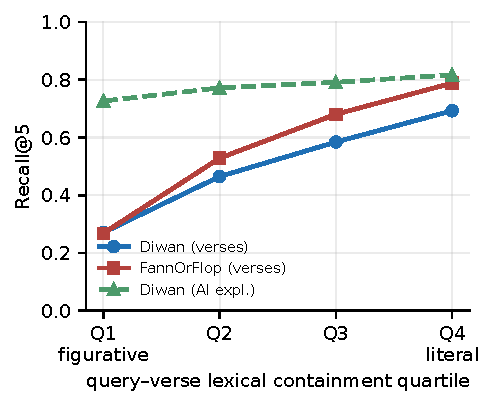
\includegraphics[width=\columnwidth]{figures/fig_mechanism_a.pdf}\\[6pt]
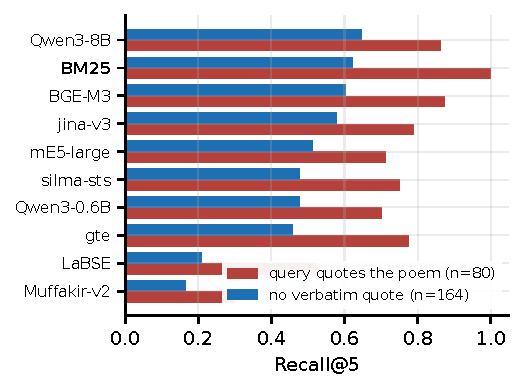
\includegraphics[width=\columnwidth]{figures/fig_mechanism_b.pdf}
\caption{Top: Verse-mode Recall@5 rises monotonically with query--verse containment on both corpora; AI explanations flatten the curve on \textit{Diwan}. Bottom: The same systems on \textit{Fann or Flop}, split by whether the query quotes the poem. BM25 is perfect with quotation and has the steepest fall without it; every system falls.}
\label{fig:mech}
\end{figure}

\section{Track B: Thematic Retrieval}
\label{sec:trackb}

Track A measures whether a system can recover a specific poem, but it cannot say whether retrieved poems are actually about what was asked. That is what an exploratory user wants, and it is what Track B evaluates. Here we score each system's top-3 results on the 200 blind thematic queries, for which no gold poem exists, using Gemini 3.5 Flash as judge on seven 1--5 aspects. All Track B claims are restricted to verse mode, where no model-generated text is shown to the judge, so self-preference toward our own AI explanations, which a different version of the same model family generated, cannot arise.

\paragraph{The judge agrees with blind human judgments.} Twenty thematic queries were pooled across
BM25, jina-v3 and their fusion, deduplicated to 126 poems, shuffled with system identity removed,
and graded by two authors independently, who were told that lexical overlap is not evidence of
relevance (Appendix~\ref{app:human}). The raters agree moderately (quadratic-weighted
$\kappa{=}0.53$, $90\%$ within one point). Across the 40 system-query cells covered by both, the
first rater's grades and the judge's overall-quality score agree strongly (Spearman $\rho{=}0.75$,
$p{=}2\times10^{-8}$; $\rho{=}0.64$ for the second rater), and both raters rank the annotated
systems as the judge does. Human raters who ignore surface matching reach the judge's ordering,
which argues against the concern that the rubric alone produces it.

\paragraph{Results.} Table~\ref{tab:trackb} gives Track B scores for all ten systems on both
corpora, complete-case over all 200 queries with no judge failures. The picture is the reverse of
Track A's. \textbf{BM25 is last of ten on both corpora} ($1.90$ on \textit{Fann or Flop}, $1.70$ on
\textit{Diwan}), and is beaten significantly by eight of the nine dense encoders on each (paired
Wilcoxon, Holm-corrected; $\Delta$ up to $-1.04$ against Qwen3-8B, $p{=}2\times10^{-18}$). The
exception on both corpora is LaBSE, the weakest dense encoder, which BM25 is statistically
indistinguishable from ($p{=}.35$ on \textit{Diwan}, $p{=}.054$ on \textit{Fann or Flop}). The blind
human judgments give the same ordering on the systems they cover: on \textit{Fann or Flop}, jina-v3
$0.93$, the RRF hybrid $0.83$, BM25 $0.50$ for the first rater (paired Wilcoxon BM25 vs.\ jina-v3
$p{=}.016$; pooled over both corpora $\Delta{=}{-}0.45$, $p{=}.005$, and $p{=}.028$ for the second
rater).

\paragraph{Two open-weights judges replicate it.} A proprietary judge cannot be re-run once
withdrawn, so we repeat Track B locally over a random half of the thematic queries ($2{,}000$ cells
per judge). The second judge, Gemma-3-27B-it, uses the identical rubric. It agrees with the primary
judge at the cell level (Spearman $\rho{=}0.67$ on overall quality) and on system ordering (Kendall
$\tau{=}{+}0.85$ on \textit{Diwan}, ${+}0.81$ on \textit{Fann or Flop}), and it tracks the blind
human judgments too ($\rho{=}0.70$). Under it BM25 is \emph{ninth} of ten rather than last, still
significantly below eight of nine dense encoders on both corpora, displaced by LaBSE, the one
system the primary judge could not separate from BM25 either. Both of these judges are Google
models, so the third, Qwen3-32B, comes from another family. It also places BM25 ninth of ten on
both corpora, above LaBSE only ($\tau{=}0.67$ and $0.89$ with the primary judge). We then remove
the literal-match aspect and its framing from the rubric and change nothing else. Under this
neutral rubric BM25 is tenth on \textit{Fann or Flop} and ninth on \textit{Diwan}, and the ordering
barely moves ($\tau{=}0.90$ and $0.97$ against the original rubric). Dropping the aspect raises
every system's score, BM25's the least ($+0.10$ against up to $+0.27$). The literal-match aspect is
therefore not what places BM25 near the bottom (Appendix~\ref{app:judge2}).

\paragraph{The judge separates matching from aboutness.} BM25 is last of ten on every aspect
requiring knowledge of what a poem is about, with its largest deficits on metaphor understanding and
semantic coverage; but on \emph{direct textual relevance}, which measures how far retrieved poems
merely repeat the query's wording, it is \emph{first} of ten on both corpora ($4.26$, $4.48$;
second of ten under the second judge, behind LaBSE; Appendix~\ref{app:aspects}). The judge
identifies BM25 as the most surface-matching system while ranking it last overall. This supports
\S\ref{sec:bridge} through a channel that shares nothing with our lexical statistics, and it argues
against the reading that the judge merely penalises lexical retrieval.

\begin{table}[t]
\centering\small
\setlength{\tabcolsep}{3.5pt}
\begin{tabular}{l cc c cc}
\toprule
& \multicolumn{2}{c}{\textit{FannOrFlop}} & & \multicolumn{2}{c}{\textit{Diwan}} \\
\cmidrule(lr){2-3}\cmidrule(lr){5-6}
System & Track A & Track B & & Track A & Track B \\
\midrule
Qwen3-8B & 0.717 & 2.94 & & 0.748 & 2.83 \\
BGE-M3 & 0.693 & 2.47 & & 0.574 & 2.29 \\
mE5-large & 0.578 & 2.52 & & 0.585 & 2.35 \\
jina-v3 & 0.647 & 2.64 & & 0.523 & 2.53 \\
silma-sts & 0.566 & 2.75 & & 0.558 & 2.63 \\
gte & 0.561 & 2.37 & & 0.488 & 2.18 \\
Qwen3-0.6B & 0.549 & 2.35 & & 0.527 & 2.14 \\
LaBSE & 0.311 & 2.07 & & 0.368 & 1.75 \\
Muffakir-v2 & 0.209 & 2.43 & & 0.233 & 2.27 \\
\midrule
\textbf{BM25} & 0.746 & 1.90 & & 0.392 & 1.70 \\
\midrule
\multicolumn{6}{l}{\textit{blind human relevance of top-3 (0 to 2), 20 queries}} \\
jina-v3 & \multicolumn{2}{c}{0.93} & & \multicolumn{2}{c}{0.87} \\
hybrid & \multicolumn{2}{c}{0.83} & & \multicolumn{2}{c}{0.57} \\
\textbf{BM25} & \multicolumn{2}{c}{0.50} & & \multicolumn{2}{c}{0.40} \\
\bottomrule
\end{tabular}
\caption{Track A (known-item Recall@5) beside Track B (thematic judge score, 1 to 5), verse mode,
$n{=}200$ queries per cell with no judge failures. The lower block gives the first rater's blind
human relevance of the top-3 (0 to 2) for the three annotated systems.}
\label{tab:trackb}
\end{table}


\section{The Dissociation}
\label{sec:dissoc}

Tracks A and B measure the same ten systems, in the same indexing mode, over the same corpora. They do not agree, and the disagreement falls where the mechanism predicts. On \textit{Fann or Flop}, BM25 ranks first of ten on Track A and last of ten on Track B, a shift of nine places (Figure~\ref{fig:dissoc}). No other system moves more than four. On \textit{Diwan}, where queries carry no remembered wording, BM25 is poor under both protocols and the ranks broadly agree. The dissociation is a property of the tip-of-the-tongue regime, not of BM25 in general.

Correlating the two rankings gives Kendall $\tau{=}+0.24$ ($p{=}0.38$) on \textit{Fann or Flop}
against $\tau{=}+0.51$ ($p{=}0.047$) on \textit{Diwan}. We do not read the first as evidence that
the protocols are unrelated in general: with ten systems one outlier is enough to move $\tau$, and
removing BM25 restores agreement ($\tau{=}+0.56$, $p{=}0.045$). Among dense encoders the protocols
largely concur; what dissociates is the lexical system, and only where remembered wording lets
surface matching succeed without any notion of aboutness.

The two results are consistent. Track A rewards recovering a specific remembered item, and where the query carries the item's wording, surface matching is close to sufficient. Track B asks whether retrieved poems are about a theme that is never stated in the poems' own words, and there surface matching has nothing to work with. Both protocols are valid, but they measure different things, and a system's score under one carries little information about its score under the other.

Reporting a single protocol can therefore mislead. A study that evaluated only known-item retrieval on a tip-of-the-tongue query set would conclude that dense retrieval is not worth its cost for Arabic poetry, since a bag of words beats a state-of-the-art 8B encoder. A study that evaluated only thematic relevance would conclude the opposite, with BM25 last of ten and significantly behind eight of the nine dense encoders. Each conclusion is supported by its own data, and neither holds in general.

\begin{figure}[t]
\centering
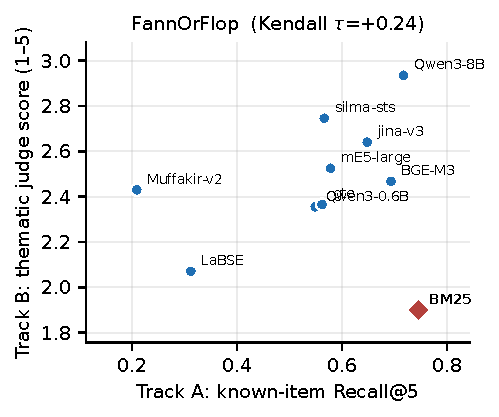
\includegraphics[width=\columnwidth]{figures/fig_dissociation_a.pdf}\\[6pt]
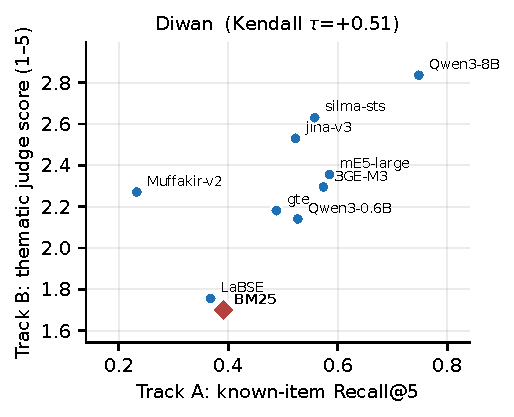
\includegraphics[width=\columnwidth]{figures/fig_dissociation_b.pdf}
\caption{The dissociation. Each point is a system; $x$ is known-item Recall@5, $y$ is the thematic
judge score. Top: on \textit{Fann or Flop}, BM25 (red diamond) is the best system on one axis and
the worst on the other. Bottom: on \textit{Diwan}, where no query carries remembered wording, the
two protocols broadly agree.}
\label{fig:dissoc}
\end{figure}


\section{Fusion and Deployment}
\label{sec:recipe}

If the query register decides which signal is useful, a practical system should combine signals rather than choose one. We test reciprocal-rank fusion \citep{cormack2009rrf} over a verse index, an explanation index and a BM25 arm (Appendix~\ref{app:fusion}, strongest encoder). Fusing explanations with verses helps everywhere, making it a safe default. Adding a lexical arm does not. Comparing the best configuration that includes a BM25 arm against the best that excludes one, the lexical arm is worth $+6.1$ points on \textit{Fann or Flop} ($0.885$ vs.\ $0.824$) and costs $9.7$ on \textit{Diwan} ($0.833$ vs.\ $0.930$, where the explanation index alone is best). The best \textit{Fann or Flop} configuration reaches $0.885$, against $0.746$ for the best single system.

No single recipe dominates, and that is the point: an archive serving readers who half-remember lines should keep a lexical arm; one serving thematic browsing should not.


\section{Discussion}
\label{sec:discussion}

Our results reframe what a benchmark number means for this task. A single Recall@5 figure for "semantic search over Arabic poetry" is not a property of a system. It is a joint property of the system and the register of the queries it was measured on, and the two standard protocols in use disagree on the same systems.

On the benchmarking side, query provenance must be reported and, ideally, manipulated. The verbatim-overlap statistic we use costs nothing to compute and would have exposed the confound in our own earlier analysis; we recommend reporting it alongside any known-item result on literary text. Known-item retrieval and thematic relevance should also be reported together, since each alone supports a defensible but opposite claim about whether dense retrieval is worth its cost.

On the modelling side, the frontier is measurable. Current encoders are strong when queries are abstract, but an 8B model still cannot beat a bag of words when the query carries remembered wording, because surface matching is nearly optimal there. The interesting residual is the non-quoting, most figurative queries, where the best system reaches roughly $0.65$, and our benchmark isolates that slice.

\section{Conclusion}

We presented the first systematic study we know of for retrieval over Classical Arabic poetry. Which retriever wins, and whether explanation augmentation helps, is governed by how much of a poem's wording the query still carries: a lexical retriever's dependence on it is significantly steeper than any dense encoder's, so a corpus-level ranking reports its query mix as much as its systems. The two protocols dissociate, reproduced by human judgments and a second judge.

\section*{Limitations}

Known-item evaluation assumes one correct poem per query, and in a corpus of this size an abstract query may plausibly describe several. We measured this rather than asserting it. On $50$ queries where the strongest system missed the gold poem, a blind annotator judged that system's top-1 result a fully acceptable answer to the query in $34\%$ of cases (95\% CI $[22,48]$) and at least partly acceptable in $72\%$. Twelve control items in which the gold poem itself was shown, shuffled indistinguishably among the rest, were scored fully acceptable in $11$ of $12$, so the annotator was discriminating rather than lenient. The rate is higher on the abstract corpus ($0.40$) than on the tip-of-the-tongue one ($0.28$). Applying each corpus its own rate, absolute Recall is conservative by eight to ten points for the best system ($0.717\!\rightarrow\!0.796$ on \textit{Fann or Flop}, $0.748\!\rightarrow\!0.849$ on \textit{Diwan}, strict criterion). Because the rate is higher where queries are abstract, the correction compresses the quotation slope of \S\ref{sec:bridge}: applying it leaves the interaction positive and ordered the same way ($+0.11$ against an uncorrected $+0.16$), though a benchmark with exhaustive relevance labels would show a smaller effect than we report. Both query sets were written by the authors rather than elicited from real users. The tip-of-the-tongue set simulates remembered wording, and the abstract set reflects one team's notion of abstractness, so while the query-abstraction spectrum is real and measured, its endpoints are constructed.

On the evaluation side, the human annotation covers 20 queries and 126 items with a single annotator, who is one of the authors. This is sufficient to confirm the direction of the Track B result but not to support fine-grained comparisons, and it carries no inter-annotator agreement. The second judge covers half the thematic queries rather than all of them, and the two judges agree least on exactly the two aspects that call for the most interpretation (metaphor understanding, literal match), so per-aspect claims are weaker than the overall ordering. The \textit{Diwan} sample is balanced across frequent poets and does not represent the full 14M-verse corpus. Finally, AI explanations were generated by a single model, and we did not test generator independence, though the fact that BM25 reproduces the same augmentation pattern without any sensitivity to explanation quality suggests that the effect is not generator-driven.

A note on the reproducibility of judged evaluation. Gemini 2.0 Flash, which generated our explanations, was withdrawn from the API during this work; an earlier round of judgments made with it can no longer be reproduced with the model that produced them. Any result that rests on a proprietary judge has this expiry property, which is an argument for releasing per-query judge outputs rather than judge scores, and for validating a judge against human annotation rather than against its own consistency. We release all per-query judge outputs and ranked lists accordingly.


\section*{Ethical Considerations}

This work supports the preservation, exploration and teaching of Classical Arabic poetry. Automated retrieval and model-generated explanations can misread metaphorical, religious or culturally sensitive language; our own analysis shows that current systems often match on surface form rather than meaning, so such tools should aid rather than replace human literary expertise. Our \textit{Diwan} sample over-represents frequently anthologised poets and may underperform on marginal traditions. Annotation was performed by an author; no external annotators were recruited or compensated.

\section*{AI Usage Disclosure}

AI assistants were used for coding support and for drafting and editing prose. All experiments were designed and run by the authors, and every number in this paper is recomputed from per-query logs by the released scripts.

% NOTE: acl.sty already issues \bibliographystyle{acl_natbib}. Declaring it again here puts a
% second \bibstyle in main.aux, which makes BibTeX abort and silently ships a PDF with no
% References section. That is what happened to a previous submission of this paper.
\bibliography{refs}

\appendix

\section{Reproducibility}
\label{app:repro}
Code, per-query ranked lists, both judges' per-query outputs, the annotation and spot-check guidelines with their completed judgments, and the query benchmark are available at \url{ANONYMOUS-URL-PLACEHOLDER}.\footnote{Anonymised repository; the de-anonymised link will replace it at camera-ready.} Every number is recomputed from per-query rank dumps by released scripts. The pipeline emits one file per (system, corpus, indexing mode, query set) containing the top-100 poem ids, scores and the rank of the gold poem; all metrics, confidence intervals, significance tests, stratifications, fusion variants and figures are derived from those files.

\section{Normalisation Ablation}
\label{app:norm}
Measured on \textit{Diwan}, verse mode, under three settings: raw text with diacritics retained; light normalisation, stripping diacritics and tatweel; and full normalisation, which additionally unifies \textit{alef}/\textit{ya}/\textit{ta-marbuta} and deletes non-Arabic characters.

\begin{center}\small
\begin{tabular}{lccc}
\toprule
Recall@5 & raw & light & full \\
\midrule
jina-v3 & 0.178 & \textbf{0.523} & 0.434 \\
gte & 0.023 & \textbf{0.488} & 0.469 \\
LaBSE & 0.093 & \textbf{0.368} & 0.333 \\
\bottomrule
\end{tabular}
\end{center}

Two conclusions, of different strength. Diacritic removal is essential, and the effect is very large and consistent across all three encoders ($+27$ to $+47$ Recall@5 points), which is unsurprising: \textit{Diwan} verses are diacritised and the models' subword vocabularies are not. The further orthographic unification points the same way for all three but varies in size by a factor of four, costing $8.9$ points on jina-v3, $3.5$ on LaBSE and $1.9$ on gte. It is also not uniformly harmful: gte's Recall@1 improves under it ($0.256\!\rightarrow\!0.318$) while LaBSE's falls ($0.209\!\rightarrow\!0.167$). We therefore apply light normalisation to every dense encoder, which is the better Recall@5 setting for all three, and full normalisation to BM25 and the lexical overlap measures, where collapsing orthographic variants is standard. An earlier version of this appendix generalised the nine-point figure to dense encoders as a class from jina-v3 alone; that generalisation is not supported.

\section{Which Overlap Measure Predicts}
\label{app:pred}
Figure~\ref{fig:pred} shows, per system, the within-query Spearman correlation between the change in query--document overlap induced by an explanation and the change in retrieval success, under a lexical and an embedding measure (\textit{Diwan}, AI-explanation mode). BM25 is the only system for which the lexical measure is the stronger predictor.

Among dense encoders on \textit{Diwan}, the more capable the model, the less its behaviour is governed by surface overlap ($\rho=-0.73$ between verse-mode Recall@5 and lexical $\rho$, $p=.025$, $n=9$). This does not hold on \textit{Fann or Flop} ($p>0.5$), so it is a property of the abstract-query regime only, and it rests on nine points.

One caveat on the embedding measure. It is computed with a single fixed encoder (gte) for every system, so that all systems are scored on the same axis. gte is itself one of the ten systems, and its own $\rho_{\mathrm{emb}}$ is consequently the highest in all three settings ($0.60$, $0.56$, $0.57$ against a next-highest of $0.50$, $0.41$, $0.38$); that row is not independent of the measure and should not be read as evidence about gte. Every conclusion above survives dropping it: the embedding measure still predicts better for the remaining eight dense encoders on \textit{Diwan} and seven of eight on \textit{Fann or Flop}, and BM25 remains the only system whose behaviour the lexical measure predicts best, with a lexical $\rho$ above every dense encoder's.

\begin{figure}[h]
\centering
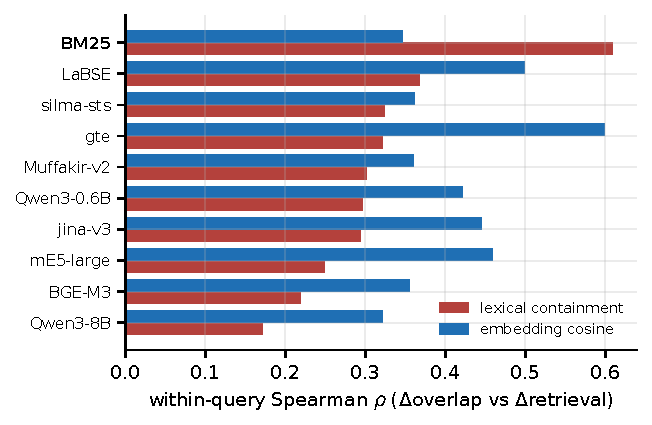
\includegraphics[width=\columnwidth]{figures/fig_predictors.pdf}
\caption{Within-query $\rho$ per system under a lexical and an embedding overlap measure.}
\label{fig:pred}
\end{figure}

\section{Multiple Comparisons}
\label{app:mult}
We report $57$ hypothesis tests in six families: the mode contrasts of Table~\ref{tab:main} (one family per corpus and contrast, ten systems each), the quotation-slope differences of \S\ref{sec:bridge} (nine systems against the reference encoder), and the Track~B comparisons of BM25 against each dense encoder (one family per corpus). Holm-Bonferroni correction within each family leaves $36$ of the $39$ nominally significant tests significant. The three that do not survive are all \textit{Fann or Flop} AI-explanation contrasts, for BGE-M3 ($p{=}.009\!\rightarrow\!.051$), mE5-large ($.033\!\rightarrow\!.136$) and Muffakir-v2 ($.027\!\rightarrow\!.136$); Table~\ref{tab:main} shows them unstarred. No claim in the paper depends on them. The interaction of \S\ref{sec:bridge} is the smallest $p$-value in its family, so Holm and Bonferroni coincide there at $p{=}.045$. Per-test and corrected values for all $57$ are released as \texttt{eacl\_multiplicity.csv}.

\section{Fusion Configurations}
\label{app:fusion}
Table~\ref{tab:fusion} gives Recall@5 for every reciprocal-rank fusion configuration we tested, for the strongest encoder.

\begin{table}[h]
\centering\small
\setlength{\tabcolsep}{3.5pt}
\begin{tabular}{l ccc c c}
\toprule
& \multicolumn{3}{c}{\textit{FannOrFlop}} & & \textit{Diwan} \\
\cmidrule(lr){2-4}\cmidrule(lr){6-6}
Index configuration & all & quote & no-qt. & & all \\
\midrule
verses only & 0.717 & 0.863 & 0.646 & & 0.748 \\
AI expl.\ only & 0.656 & 0.713 & 0.628 & & 0.930 \\
FoF expl.\ only & 0.816 & 0.812 & 0.817 & & n/a \\
vrs.\,$\oplus$\,AI expl. & 0.730 & 0.800 & 0.695 & & 0.857 \\
vrs.\,$\oplus$\,FoF expl. & 0.824 & 0.912 & 0.780 & & n/a \\
vrs.\,$\oplus$\,BM25 & 0.836 & 1.000 & 0.756 & & 0.616 \\
vrs.\,$\oplus$\,BM25\,$\oplus$\,AI expl. & 0.873 & 1.000 & 0.811 & & 0.833 \\
vrs.\,$\oplus$\,BM25\,$\oplus$\,FoF expl. & 0.885 & 0.988 & 0.835 & & n/a \\
\bottomrule
\end{tabular}
\caption{Reciprocal-rank fusion over index configurations, Qwen3-8B. $\oplus$ denotes RRF ($k{=}60$). Fusing explanations is safe everywhere; adding a lexical arm helps only where queries carry remembered wording.}
\label{tab:fusion}
\end{table}

\section{Threshold Robustness of the Controlled Split}
\label{app:threshold}
\S\ref{sec:bridge} splits \textit{Fann or Flop} on whether the query shares a verbatim three-token span with the target poem. Table~\ref{tab:appthreshold} repeats the split at spans of two to five tokens. Two things are stable: BM25 retrieves the gold poem within the top five for \emph{every} quoting query at the three-, four- and five-token thresholds (and for $140$ of $146$ at two tokens), and its quotation slope stays significantly steeper than Qwen3-8B's ($p{=}.0001$, $.005$, $.006$, $.049$ for thresholds two to five). The non-quoting comparison behaves as the graded account predicts: at a two-token threshold the non-quoting subset is the most abstract and Qwen3-8B leads it significantly ($0.571$ vs.\ $0.429$, $p{=}.039$); as the threshold rises, queries with two- and three-token overlaps re-enter the non-quoting subset and the gap closes to parity. Note that BM25's slope is bounded above by its perfect quoting-subset score, so at the four- and five-token thresholds, where its non-quoting score has risen to $0.70$--$0.72$, three weaker encoders show nominally larger slopes; its slope remains significantly larger than that of the strongest dense encoder throughout.

\begin{table}[h]
\centering\scriptsize
\setlength{\tabcolsep}{2.5pt}
\begin{tabular}{lcccccccc}
\toprule
& \multicolumn{2}{c}{$\geq2$} & \multicolumn{2}{c}{$\geq3$} & \multicolumn{2}{c}{$\geq4$} & \multicolumn{2}{c}{$\geq5$} \\
\cmidrule(lr){2-3}\cmidrule(lr){4-5}\cmidrule(lr){6-7}\cmidrule(lr){8-9}
System & qt. & no-qt. & qt. & no-qt. & qt. & no-qt. & qt. & no-qt. \\
& \scriptsize 146 & \scriptsize 98 & \scriptsize 80 & \scriptsize 164 & \scriptsize 40 & \scriptsize 204 & \scriptsize 24 & \scriptsize 220 \\
\midrule
Qwen3-8B & 0.815 & 0.571 & 0.863 & 0.646 & 0.825 & 0.696 & 0.833 & 0.705 \\
BGE-M3 & 0.856 & 0.449 & 0.875 & 0.604 & 0.950 & 0.642 & 0.958 & 0.664 \\
mE5-large & 0.678 & 0.429 & 0.713 & 0.512 & 0.775 & 0.539 & 0.917 & 0.541 \\
jina-v3 & 0.801 & 0.418 & 0.787 & 0.579 & 0.850 & 0.608 & 0.917 & 0.618 \\
silma-sts & 0.692 & 0.378 & 0.750 & 0.476 & 0.725 & 0.534 & 0.792 & 0.541 \\
gte & 0.753 & 0.276 & 0.775 & 0.457 & 0.850 & 0.505 & 0.917 & 0.523 \\
Qwen3-0.6B & 0.678 & 0.357 & 0.700 & 0.476 & 0.775 & 0.505 & 0.833 & 0.518 \\
LaBSE & 0.445 & 0.112 & 0.525 & 0.207 & 0.600 & 0.255 & 0.667 & 0.273 \\
Muffakir-v2 & 0.281 & 0.102 & 0.300 & 0.165 & 0.275 & 0.196 & 0.292 & 0.200 \\
\midrule
\textbf{BM25} & 0.959 & 0.429 & 1.000 & 0.622 & 1.000 & 0.696 & 1.000 & 0.718 \\
\bottomrule
\end{tabular}

\caption{Verse-mode Recall@5 on \textit{Fann or Flop}, split at verbatim spans of $\geq$2 to $\geq$5 tokens. Subset sizes are given under each threshold.}
\label{tab:appthreshold}
\end{table}

\section{Full Track A Results}
\label{app:full}
Table~\ref{tab:apptracka} gives Recall@1/@5, MRR and nDCG@10 with bootstrap 95\% confidence intervals ($10^4$ resamples) for every system, corpus and indexing mode. Per-subset results are released with the code as \texttt{eacl\_trackA.csv}.

\begin{table*}[t]
\centering\scriptsize
\setlength{\tabcolsep}{3pt}
\begin{tabular}{ll cccc}
\toprule
System & Mode & R@1 & R@5 & MRR & nDCG@10 \\
\midrule
\multicolumn{6}{l}{\textit{Fann or Flop}} \\
Qwen3-8B & verses & 0.566 \scriptsize [0.504,0.627] & 0.717 \scriptsize [0.660,0.770] & 0.635 \scriptsize [0.581,0.688] & 0.667 \scriptsize [0.615,0.718] \\
Qwen3-8B & AI expl. & 0.426 \scriptsize [0.365,0.488] & 0.656 \scriptsize [0.594,0.713] & 0.530 \scriptsize [0.475,0.584] & 0.570 \scriptsize [0.517,0.622] \\
Qwen3-8B & FoF expl. & 0.639 \scriptsize [0.578,0.701] & 0.816 \scriptsize [0.766,0.865] & 0.725 \scriptsize [0.677,0.773] & 0.754 \scriptsize [0.710,0.800] \\
BGE-M3 & verses & 0.574 \scriptsize [0.512,0.635] & 0.693 \scriptsize [0.635,0.750] & 0.634 \scriptsize [0.578,0.689] & 0.657 \scriptsize [0.603,0.712] \\
BGE-M3 & AI expl. & 0.406 \scriptsize [0.344,0.467] & 0.598 \scriptsize [0.537,0.660] & 0.489 \scriptsize [0.434,0.544] & 0.515 \scriptsize [0.459,0.570] \\
BGE-M3 & FoF expl. & 0.566 \scriptsize [0.504,0.627] & 0.725 \scriptsize [0.668,0.779] & 0.646 \scriptsize [0.593,0.699] & 0.676 \scriptsize [0.624,0.727] \\
mE5-large & verses & 0.414 \scriptsize [0.352,0.475] & 0.578 \scriptsize [0.516,0.639] & 0.485 \scriptsize [0.429,0.542] & 0.510 \scriptsize [0.454,0.566] \\
mE5-large & AI expl. & 0.332 \scriptsize [0.275,0.389] & 0.492 \scriptsize [0.430,0.553] & 0.408 \scriptsize [0.355,0.464] & 0.437 \scriptsize [0.382,0.492] \\
mE5-large & FoF expl. & 0.557 \scriptsize [0.492,0.619] & 0.717 \scriptsize [0.660,0.770] & 0.632 \scriptsize [0.576,0.685] & 0.662 \scriptsize [0.611,0.714] \\
jina-v3 & verses & 0.479 \scriptsize [0.418,0.541] & 0.647 \scriptsize [0.586,0.705] & 0.559 \scriptsize [0.502,0.614] & 0.589 \scriptsize [0.533,0.643] \\
jina-v3 & AI expl. & 0.303 \scriptsize [0.246,0.361] & 0.504 \scriptsize [0.439,0.566] & 0.395 \scriptsize [0.343,0.449] & 0.430 \scriptsize [0.377,0.486] \\
jina-v3 & FoF expl. & 0.512 \scriptsize [0.451,0.574] & 0.676 \scriptsize [0.615,0.734] & 0.592 \scriptsize [0.538,0.645] & 0.623 \scriptsize [0.569,0.676] \\
silma-sts & verses & 0.389 \scriptsize [0.332,0.451] & 0.566 \scriptsize [0.504,0.627] & 0.479 \scriptsize [0.424,0.532] & 0.511 \scriptsize [0.455,0.566] \\
silma-sts & AI expl. & 0.361 \scriptsize [0.299,0.422] & 0.508 \scriptsize [0.447,0.570] & 0.439 \scriptsize [0.384,0.495] & 0.475 \scriptsize [0.419,0.529] \\
silma-sts & FoF expl. & 0.516 \scriptsize [0.451,0.578] & 0.717 \scriptsize [0.660,0.775] & 0.606 \scriptsize [0.552,0.659] & 0.641 \scriptsize [0.590,0.694] \\
gte & verses & 0.439 \scriptsize [0.377,0.500] & 0.561 \scriptsize [0.500,0.623] & 0.504 \scriptsize [0.448,0.561] & 0.532 \scriptsize [0.477,0.589] \\
gte & AI expl. & 0.254 \scriptsize [0.201,0.307] & 0.389 \scriptsize [0.328,0.451] & 0.331 \scriptsize [0.280,0.382] & 0.356 \scriptsize [0.304,0.409] \\
gte & FoF expl. & 0.459 \scriptsize [0.398,0.520] & 0.635 \scriptsize [0.574,0.693] & 0.541 \scriptsize [0.485,0.596] & 0.569 \scriptsize [0.513,0.624] \\
Qwen3-0.6B & verses & 0.414 \scriptsize [0.352,0.475] & 0.549 \scriptsize [0.488,0.611] & 0.484 \scriptsize [0.427,0.542] & 0.509 \scriptsize [0.452,0.566] \\
Qwen3-0.6B & AI expl. & 0.266 \scriptsize [0.213,0.324] & 0.430 \scriptsize [0.369,0.492] & 0.346 \scriptsize [0.294,0.398] & 0.376 \scriptsize [0.323,0.429] \\
Qwen3-0.6B & FoF expl. & 0.455 \scriptsize [0.393,0.516] & 0.660 \scriptsize [0.598,0.721] & 0.552 \scriptsize [0.498,0.608] & 0.590 \scriptsize [0.537,0.643] \\
LaBSE & verses & 0.197 \scriptsize [0.147,0.250] & 0.311 \scriptsize [0.254,0.373] & 0.253 \scriptsize [0.205,0.303] & 0.272 \scriptsize [0.223,0.322] \\
LaBSE & AI expl. & 0.189 \scriptsize [0.139,0.238] & 0.283 \scriptsize [0.225,0.340] & 0.237 \scriptsize [0.189,0.286] & 0.248 \scriptsize [0.199,0.298] \\
LaBSE & FoF expl. & 0.213 \scriptsize [0.164,0.266] & 0.336 \scriptsize [0.275,0.394] & 0.274 \scriptsize [0.224,0.324] & 0.298 \scriptsize [0.247,0.350] \\
Muffakir-v2 & verses & 0.107 \scriptsize [0.070,0.147] & 0.209 \scriptsize [0.160,0.262] & 0.167 \scriptsize [0.128,0.208] & 0.185 \scriptsize [0.145,0.227] \\
Muffakir-v2 & AI expl. & 0.172 \scriptsize [0.127,0.221] & 0.287 \scriptsize [0.234,0.344] & 0.236 \scriptsize [0.191,0.282] & 0.260 \scriptsize [0.213,0.309] \\
Muffakir-v2 & FoF expl. & 0.324 \scriptsize [0.266,0.385] & 0.467 \scriptsize [0.406,0.529] & 0.399 \scriptsize [0.345,0.455] & 0.427 \scriptsize [0.374,0.483] \\
\textbf{BM25} & verses & 0.656 \scriptsize [0.594,0.717] & 0.746 \scriptsize [0.689,0.799] & 0.699 \scriptsize [0.644,0.751] & 0.720 \scriptsize [0.667,0.770] \\
\textbf{BM25} & AI expl. & 0.246 \scriptsize [0.193,0.303] & 0.357 \scriptsize [0.299,0.418] & 0.301 \scriptsize [0.249,0.354] & 0.323 \scriptsize [0.271,0.377] \\
\textbf{BM25} & FoF expl. & 0.603 \scriptsize [0.541,0.664] & 0.742 \scriptsize [0.684,0.795] & 0.665 \scriptsize [0.611,0.718] & 0.690 \scriptsize [0.635,0.740] \\
\midrule
\multicolumn{6}{l}{\textit{Diwan}} \\
Qwen3-8B & verses & 0.527 \scriptsize [0.469,0.585] & 0.748 \scriptsize [0.694,0.798] & 0.629 \scriptsize [0.580,0.681] & 0.667 \scriptsize [0.618,0.713] \\
Qwen3-8B & AI expl. & 0.779 \scriptsize [0.729,0.830] & 0.930 \scriptsize [0.895,0.961] & 0.849 \scriptsize [0.812,0.885] & 0.871 \scriptsize [0.837,0.903] \\
BGE-M3 & verses & 0.403 \scriptsize [0.341,0.461] & 0.574 \scriptsize [0.512,0.632] & 0.488 \scriptsize [0.436,0.542] & 0.521 \scriptsize [0.467,0.576] \\
BGE-M3 & AI expl. & 0.686 \scriptsize [0.632,0.740] & 0.845 \scriptsize [0.798,0.888] & 0.752 \scriptsize [0.705,0.797] & 0.779 \scriptsize [0.735,0.822] \\
mE5-large & verses & 0.353 \scriptsize [0.298,0.411] & 0.585 \scriptsize [0.523,0.647] & 0.453 \scriptsize [0.401,0.506] & 0.492 \scriptsize [0.440,0.544] \\
mE5-large & AI expl. & 0.659 \scriptsize [0.601,0.713] & 0.802 \scriptsize [0.752,0.849] & 0.726 \scriptsize [0.676,0.774] & 0.753 \scriptsize [0.706,0.798] \\
jina-v3 & verses & 0.345 \scriptsize [0.287,0.403] & 0.523 \scriptsize [0.461,0.581] & 0.429 \scriptsize [0.378,0.482] & 0.456 \scriptsize [0.402,0.509] \\
jina-v3 & AI expl. & 0.589 \scriptsize [0.531,0.647] & 0.756 \scriptsize [0.702,0.806] & 0.667 \scriptsize [0.616,0.717] & 0.694 \scriptsize [0.645,0.742] \\
silma-sts & verses & 0.380 \scriptsize [0.322,0.438] & 0.558 \scriptsize [0.500,0.616] & 0.466 \scriptsize [0.412,0.519] & 0.500 \scriptsize [0.449,0.552] \\
silma-sts & AI expl. & 0.659 \scriptsize [0.601,0.717] & 0.810 \scriptsize [0.764,0.857] & 0.726 \scriptsize [0.677,0.775] & 0.751 \scriptsize [0.705,0.796] \\
gte & verses & 0.256 \scriptsize [0.205,0.310] & 0.488 \scriptsize [0.430,0.550] & 0.361 \scriptsize [0.313,0.411] & 0.402 \scriptsize [0.352,0.452] \\
gte & AI expl. & 0.651 \scriptsize [0.593,0.709] & 0.806 \scriptsize [0.760,0.853] & 0.724 \scriptsize [0.675,0.772] & 0.747 \scriptsize [0.700,0.792] \\
Qwen3-0.6B & verses & 0.333 \scriptsize [0.275,0.392] & 0.527 \scriptsize [0.465,0.585] & 0.429 \scriptsize [0.377,0.481] & 0.463 \scriptsize [0.411,0.516] \\
Qwen3-0.6B & AI expl. & 0.624 \scriptsize [0.566,0.682] & 0.795 \scriptsize [0.744,0.845] & 0.696 \scriptsize [0.644,0.745] & 0.723 \scriptsize [0.673,0.771] \\
LaBSE & verses & 0.209 \scriptsize [0.163,0.260] & 0.368 \scriptsize [0.310,0.426] & 0.285 \scriptsize [0.237,0.333] & 0.312 \scriptsize [0.263,0.362] \\
LaBSE & AI expl. & 0.519 \scriptsize [0.457,0.581] & 0.670 \scriptsize [0.612,0.729] & 0.592 \scriptsize [0.537,0.644] & 0.620 \scriptsize [0.567,0.671] \\
Muffakir-v2 & verses & 0.132 \scriptsize [0.093,0.174] & 0.233 \scriptsize [0.182,0.287] & 0.190 \scriptsize [0.149,0.233] & 0.206 \scriptsize [0.163,0.251] \\
Muffakir-v2 & AI expl. & 0.442 \scriptsize [0.384,0.500] & 0.585 \scriptsize [0.527,0.647] & 0.508 \scriptsize [0.452,0.564] & 0.533 \scriptsize [0.478,0.588] \\
\textbf{BM25} & verses & 0.248 \scriptsize [0.198,0.302] & 0.392 \scriptsize [0.333,0.454] & 0.321 \scriptsize [0.272,0.372] & 0.349 \scriptsize [0.298,0.401] \\
\textbf{BM25} & AI expl. & 0.612 \scriptsize [0.554,0.670] & 0.760 \scriptsize [0.709,0.810] & 0.676 \scriptsize [0.624,0.726] & 0.698 \scriptsize [0.648,0.747] \\
\bottomrule
\end{tabular}

\caption{Track A in full, with bootstrap 95\% confidence intervals.}
\label{tab:apptracka}
\end{table*}

\section{The Second Judge}
\label{app:judge2}
Track B was repeated with Gemma-3-27B-it, quantised to 4 bits and run on one consumer GPU, over a random $100$ of the $200$ thematic queries for all ten systems and both corpora ($2{,}000$ cells, no parse failures). The rubric text is identical to the primary judge's; only the response format differs, in that the second judge returns the seven scores with a single short justification rather than seven, which keeps local decoding tractable. Table~\ref{tab:appjudge2} gives system means under both judges and Table~\ref{tab:appjudge2rho} the cell-level agreement per aspect.

Agreement is high on the five aspects that ask about aboutness ($\rho$ between $0.65$ and $0.71$) and much lower on metaphor understanding ($0.26$) and literal match ($0.29$). We take this at face value: the two aspects on which the judges agree least are the two that ask for the most interpretive judgement, and conclusions that rest on them are correspondingly weaker. The overall-quality ordering, which carries the Track B claim, is not one of them.

\begin{table}[h]
\centering\small
\setlength{\tabcolsep}{4pt}
\begin{tabular}{l cc c cc}
\toprule
& \multicolumn{2}{c}{\textit{FannOrFlop}} & & \multicolumn{2}{c}{\textit{Diwan}} \\
\cmidrule(lr){2-3}\cmidrule(lr){5-6}
System & judge 1 & judge 2 & & judge 1 & judge 2 \\
\midrule
Qwen3-8B & 2.83 & 3.36 & & 2.68 & 3.29 \\
BGE-M3 & 2.49 & 3.09 & & 2.34 & 3.00 \\
mE5-large & 2.48 & 3.23 & & 2.36 & 3.18 \\
jina-v3 & 2.51 & 3.19 & & 2.48 & 3.18 \\
silma-sts & 2.73 & 3.23 & & 2.56 & 3.17 \\
gte & 2.45 & 3.04 & & 2.10 & 2.90 \\
Qwen3-0.6B & 2.32 & 3.08 & & 2.18 & 3.02 \\
LaBSE & 1.93 & 2.82 & & 1.59 & 2.58 \\
Muffakir-v2 & 2.37 & 3.02 & & 2.16 & 2.99 \\
\midrule
\textbf{BM25} & 1.96 & 2.84 & & 1.70 & 2.69 \\
\bottomrule
\end{tabular}

\caption{Track B overall quality under the primary judge (Gemini 3.5 Flash, $n{=}200$) and the open-weights second judge (Gemma-3-27B-it, $n{=}100$). Scales differ; the orderings do not (Kendall $\tau{=}{+}0.85$ and ${+}0.81$).}
\label{tab:appjudge2}
\end{table}

\begin{table}[h]
\centering\small
\begin{tabular}{lc}
\toprule
Aspect & cell-level $\rho$ \\
\midrule
semantic relevance & +0.71 \\
thematic coherence & +0.64 \\
metaphor understanding & +0.26 \\
coverage & +0.68 \\
literal match & +0.29 \\
precision & +0.65 \\
overall quality & +0.67 \\
\bottomrule
\end{tabular}

\caption{Cell-level Spearman agreement between the two judges, $n{=}2{,}000$ paired cells.}
\label{tab:appjudge2rho}
\end{table}

\section{Track B by Judge Aspect}
\label{app:aspects}
Table~\ref{tab:appaspects} breaks Track B out by all seven rubric aspects. Two patterns matter for internal validity. First, BM25 is last of ten on every aspect that requires aboutness on \textit{Fann or Flop} and on all but one on \textit{Diwan}, with its largest deficits on metaphor understanding and semantic coverage ($1.1$--$1.2$ points below the best system), which is where an aboutness-blind system should fail. Second, on \emph{direct textual relevance}, the aspect that measures how far a system's results simply repeat the query's wording, BM25 scores highest of all ten systems on both corpora ($4.26$ on \textit{Fann or Flop}, $4.48$ on \textit{Diwan}). The judge therefore identifies BM25 as the most surface-matching system while scoring it lowest overall, which is both an independent confirmation of the mechanism from a separate measurement channel and evidence that the low overall score is not an undifferentiated dislike of lexical retrieval.

\begin{table*}[t]
\centering\small
\begin{tabular}{llccccccc}
\toprule
Corpus & System & sem.\,rel. & them.\,coh. & metaph. & coverage & lit.\,match & prec. & overall \\
\midrule
FoF & Qwen3-8B & 3.00 & 2.70 & 2.94 & 3.08 & 3.27 & 2.80 & 2.94 \\
FoF & BGE-M3 & 2.54 & 2.33 & 2.55 & 2.58 & 3.25 & 2.37 & 2.47 \\
FoF & mE5-large & 2.60 & 2.46 & 2.66 & 2.58 & 3.28 & 2.37 & 2.52 \\
FoF & jina-v3 & 2.69 & 2.48 & 2.73 & 2.75 & 3.15 & 2.52 & 2.64 \\
FoF & silma-sts & 2.85 & 2.57 & 2.84 & 2.85 & 2.90 & 2.62 & 2.75 \\
FoF & gte & 2.42 & 2.21 & 2.38 & 2.46 & 3.40 & 2.22 & 2.37 \\
FoF & Qwen3-0.6B & 2.47 & 2.21 & 2.35 & 2.41 & 3.47 & 2.25 & 2.35 \\
FoF & LaBSE & 2.15 & 1.90 & 2.15 & 2.10 & 3.35 & 1.98 & 2.07 \\
FoF & Muffakir-v2 & 2.48 & 2.31 & 2.46 & 2.48 & 3.17 & 2.33 & 2.43 \\
FoF & \textbf{BM25} & 1.95 & 1.73 & 1.87 & 1.94 & 4.26 & 1.78 & 1.90 \\
\midrule
Diwan & Qwen3-8B & 3.00 & 2.65 & 2.91 & 2.89 & 3.29 & 2.77 & 2.83 \\
Diwan & BGE-M3 & 2.42 & 2.27 & 2.45 & 2.41 & 3.38 & 2.24 & 2.29 \\
Diwan & mE5-large & 2.44 & 2.29 & 2.45 & 2.40 & 3.40 & 2.21 & 2.35 \\
Diwan & jina-v3 & 2.65 & 2.44 & 2.68 & 2.60 & 3.29 & 2.45 & 2.53 \\
Diwan & silma-sts & 2.75 & 2.50 & 2.70 & 2.73 & 3.05 & 2.52 & 2.63 \\
Diwan & gte & 2.27 & 2.06 & 2.27 & 2.26 & 3.54 & 2.10 & 2.18 \\
Diwan & Qwen3-0.6B & 2.23 & 2.03 & 2.12 & 2.15 & 3.71 & 2.04 & 2.14 \\
Diwan & LaBSE & 1.86 & 1.65 & 1.82 & 1.77 & 3.76 & 1.62 & 1.75 \\
Diwan & Muffakir-v2 & 2.41 & 2.19 & 2.41 & 2.29 & 3.23 & 2.16 & 2.27 \\
Diwan & \textbf{BM25} & 1.81 & 1.64 & 1.69 & 1.74 & 4.48 & 1.65 & 1.70 \\
\bottomrule
\end{tabular}

\caption{Track B by judge aspect, verse mode, $n{=}200$ queries per cell. All aspects are scored 1--5 with 5 highest; on \textit{lit.\ match} a high score means the results repeat the query's wording, which the rubric treats as evidence \emph{against} implicit understanding.}
\label{tab:appaspects}
\end{table*}

\section{Annotation Guidelines}
\label{app:annot}
\textbf{Thematic relevance.} Annotators saw a theme and a shuffled, deduplicated pool of poems retrieved for it by several anonymised systems, and graded each poem: 2 = clearly on-theme, 1 = partly or tangentially on-theme, 0 = off-theme. The instructions stated explicitly that lexical overlap with the theme is not evidence of relevance, that a poem repeating the theme's words while being about something else scores 0, and that a poem never using them while genuinely being about the theme scores 2.

\textbf{Known-item spot check.} Each item showed one query and one retrieved poem, and asked only whether that poem would satisfy someone issuing the query: 2 = yes, 1 = partly or arguably, 0 = no. The instructions stated that the annotator would not be told which items showed the labelled gold poem and that guessing was counter-productive, and that a query may legitimately describe more than one poem, so a genuine answer scores 2 even if a different poem was intended. Both guideline documents and the completed judgments are released.

\section{LLM Prompts and Rubric}
\label{app:prompts}
\textbf{Explanation generation.} Each verse is paired with a fixed instruction asking for a concise, faithful prose paraphrase of the verse's meaning in Arabic, adding no information beyond the verse.

\textbf{Judge rubric.} The judge receives a query and the retrieved poems and scores seven 1--5 aspects, each with a one-line justification: semantic relevance, thematic coherence, metaphor understanding, semantic coverage, direct textual relevance (where 1 is best, i.e.\ least literal matching), precision, and overall quality. Exact prompt strings are released with the code.

\end{document}
